% ==========================================================================
%  SPHERExLens -- research paper (conference style, single column)
%  Build:  pdflatex spherexlens_research_paper.tex   (twice, for references)
% ==========================================================================
\documentclass[11pt,a4paper]{article}

\usepackage[T1]{fontenc}
\usepackage[utf8]{inputenc}
\usepackage{lmodern}
\usepackage[a4paper,margin=2.3cm,top=2.5cm,bottom=2.4cm]{geometry}
\usepackage{amsmath,amssymb}
\usepackage{booktabs,array,multirow}
\usepackage{graphicx}
\usepackage{xcolor}
\usepackage[font=small,labelfont=bf]{caption}
\usepackage{enumitem}
\usepackage{titlesec}
\usepackage{fancyhdr}
\usepackage{tikz}
\usetikzlibrary{arrows.meta,positioning,calc,fit,backgrounds}
\usepackage{pgfplots}
\pgfplotsset{compat=1.18}
\usepackage[hidelinks]{hyperref}
\usepackage{microtype}

\setlength{\headheight}{14pt}
\setlength{\emergencystretch}{3em}
\sloppy

\definecolor{ink}{HTML}{14213A}
\definecolor{slate}{HTML}{3F4A5A}
\definecolor{muted}{HTML}{6E7A8A}
\definecolor{accent}{HTML}{1F6FB2}
\definecolor{accent2}{HTML}{E8F1F8}
\definecolor{good}{HTML}{1E7B4F}
\definecolor{bad}{HTML}{B3261E}
\definecolor{warn}{HTML}{8A5A00}
\definecolor{rule}{HTML}{D5DAE2}

\pagestyle{fancy}
\fancyhf{}
\fancyhead[L]{\footnotesize\color{slate}SPHERExLens --- difference imaging on SPHEREx DR1}
\fancyhead[R]{\footnotesize\color{slate}\thepage}
\renewcommand{\headrulewidth}{0.4pt}

\titleformat{\section}{\large\bfseries\color{ink}}{\thesection}{0.7em}{}
\titleformat{\subsection}{\normalsize\bfseries\color{ink}}{\thesubsection}{0.6em}{}
\titlespacing*{\section}{0pt}{1.6ex plus .3ex}{0.7ex}
\titlespacing*{\subsection}{0pt}{1.2ex plus .2ex}{0.5ex}

\newcommand{\code}[1]{\texttt{\small #1}}
\newcommand{\arcsec}{\ensuremath{{}^{\prime\prime}}}
\newcommand{\arcmin}{\ensuremath{{}^{\prime}}}

\begin{document}

\begin{center}
{\LARGE\bfseries\color{ink} SPHERExLens: an open, calibrated difference-imaging\\[2pt]
pipeline for SPHEREx Data Release 1\par}
\vspace{6pt}
{\large Evan Lim \quad\textbullet\quad SPHERExLens collaboration\par}
\vspace{2pt}
{\small November 2026\par}
\end{center}

\vspace{4pt}
\begin{abstract}
\noindent
Time-domain astronomy with an all-sky infrared survey requires three things usually delivered
separately: a subtraction that is statistically understood, a triage that is reproducible, and an
implementation another group can audit. We present SPHERExLens, an end-to-end pipeline from public
SPHEREx Data Release 1 (DR1) Level-2 cut-outs to a defensible candidate list. It uses closed-form
Fourier proper subtraction (ZOGY) with empirical point-spread functions measured on a
$21\times21$ detector-zone grid, a $6.0\sigma$ threshold calibrated against split-epoch null tests,
physically constrained dipole pairing, six-way catalogue triage with proper-motion epoch
propagation, and an explainable evidence score. On 18 fields and 246 cut-outs the pipeline reports
109 detections, of which 99 (91\%) are explained by Gaia DR3, AllWISE, NEOWISE, VSX, JPL Horizons or
optical artefacts, leaving 10 candidates in five fields. Strict injection--recovery over 12\,240
planted sources reaches 69.3\% overall (96.7\% brightening, 95.3\% fading, 56.0\% moving), up from
0.2\% before the detector recalibration we describe. Split-epoch null tests over 220 realisations
give $1.66$ false candidates per field, and zero in six star fields. Every number here is
reproducible from public archives; the pipeline, harness and deployment are released openly.
\end{abstract}

\vspace{2pt}
{\small\noindent\textbf{Keywords:} methods: data analysis --- techniques: image processing ---

\section{Introduction}

A single image tells you where objects are. A second image, taken later, tells you what changed ---
and change is where most of the physics lives. Difference imaging exploits this: subtract one epoch
from another and the stationary sky --- stars, galaxies, the diffuse infrared background ---
cancels, leaving only sources that moved, brightened or faded.

The cancellation is never perfect. Two visits differ in point-spread function (PSF), detector
temperature, sub-pixel sampling and spacecraft roll. The residuals are structured and correlated,
and typically outnumber genuine astrophysical changes by two to three orders of magnitude. The
scientific problem is therefore not subtraction, which is a two-line operation, but deciding which
residuals are astrophysics at a stated false-alarm rate.

SPHEREx makes this both tractable and urgent: it images the whole sky in 102 infrared bands between
0.75 and 5.0\,\textmu m and repeats the survey every six months \cite{spherex}. Each visit is a
genuine time-domain measurement, with a baseline long enough that solar-system objects vacate the
field while variability and proper motion persist.

This paper describes SPHERExLens, an open pipeline built for that dataset. Its contributions are
(i) an end-to-end, inspectable path from public Level-2 cut-outs to a triaged candidate list, with a
single JSON contract between science stages and serving layers; (ii) a calibrated detection
statistic --- the analytic Gaussian null of ZOGY \cite{zogy}, checked and re-calibrated against
split-epoch null tests on real co-adds; (iii) a detector design (robust normalisation, physical
dipole pairing, brightness-scaled masking) validated by strict injection--recovery, improving
completeness by more than two orders of magnitude; and (iv) an explicit accounting of failure modes,
including empty fields, refused fields, and a machine-learning metric reported as inflated.

\section{Related work}

\paragraph{Image subtraction.}
Alard \& Lupton \cite{alard} introduced optimal image subtraction, fitting a spatially varying kernel
expanded in basis functions to bright reference stars. Bramich \cite{bramich} replaced the basis
expansion with a discrete per-pixel kernel. Zackay, Ofek \& Gal-Yam \cite{zogy} derived the
closed-form maximum-likelihood solution in Fourier space, producing a significance map with unit
variance wherever the sky is constant. SFFT \cite{sfft} recasts the same mathematics with a
delta-basis kernel suited to undersampled space PSFs. We adopt ZOGY because its analytic null makes
the threshold a probability statement rather than an empirical choice.

\paragraph{Brokers and triage.}
Operational surveys run a four-stage loop: detect against a template, veto with catalogues and
machine learning, triage survivors, hand candidates to a human. Brokers such as ANTARES
\cite{antares}, ALeRCE \cite{alerce}, Lasair \cite{lasair} and Fink \cite{fink} industrialise the
veto, but consume alerts produced inside their own surveys. For SPHEREx no published, inspectable,
end-to-end instance from Level-2 pixels exists. The gap is thus infrastructural rather than
algorithmic: a reproducible implementation built only from public data.

\section{Data and field sample}

\subsection{SPHEREx DR1 products}
Each cut-out is a small stamp of a much larger parent frame ($\sim$70\,MB) and carries six Level-2
FITS extensions: \code{IMAGE} (calibrated surface brightness), \code{FLAGS} (32-bit quality mask),
\code{VARIANCE}, \code{WCS-WAVE} (per-pixel wavelength solution), \code{EPSF} (empirical PSF) and
\code{ZODI} (zodiacal light model). All six are used: the PSF makes matched subtraction possible,
the flag plane prevents subtracting artefacts, and the wavelength solution yields a
low-resolution spectrum from the same cut-out.

The 102 bands span 0.75--5.0\,\textmu m through a linear variable filter, so a pixel's position on
the detector determines its wavelength. The survey cadence is six months.

\subsection{Field sample}
We evaluate 18 fields (Table~\ref{tab:fields}): five mandatory targets and thirteen benchmarks
chosen to stress different failure modes --- crowded stellar fields, extended nebulae, a bright
quasar, a globular cluster and a nearby dwarf galaxy. Cut-outs are fetched as $\sim$5\,MB stamps
through an SIA2 cone search or a direct read from the public S3 bucket, and accepted only with
$\ge$12 pixels of valid margin and $<$50\% flagged pixels. Eighteen fields yield 246 accepted
cut-outs across detector arrays D1--D6.

\begin{table}[t]
\centering
\caption{Field sample. Detections are given in the 6.0$\sigma$ census of
Section~\ref{sec:results}; ``---'' means the field was evaluated but returned no detection.}
\label{tab:fields}
\small
\begin{tabular}{@{}llrr@{}}
\toprule
Field & Role & Detections & Candidates \\
\midrule
Barnard's Star      & brief target & 9 & 0 \\
Epsilon Indi B      & brief target & 7 & 3 \\
WISE 0855           & brief target & 7 & 2 \\
TRAPPIST-1          & brief target & 5 & 2 \\
RW Aurigae          & brief target & 4 & 0 \\
M31                 & benchmark    & 10 & 0 \\
M104 (Sombrero)     & benchmark    & 8 & 0 \\
M57 (Ring Nebula)   & benchmark    & 6 & 0 \\
M1 (Crab)           & benchmark    & 6 & 0 \\
M45 (Pleiades)      & benchmark    & 9 & 2 \\
3C 273              & benchmark    & 6 & 1 \\
Sirius              & benchmark    & 6 & 0 \\
R Draconis          & benchmark    & 5 & 0 \\
Betelgeuse          & benchmark    & 4 & 0 \\
Proxima Centauri    & benchmark    & 3 & 0 \\
M42 (Orion)         & benchmark    & 0 & 0 \\
Sgr A$^{*}$         & benchmark    & 0 & 0 \\
LMC                 & benchmark    & --- & --- \\
\midrule
\textbf{Total}      & 18 fields    & \textbf{109} & \textbf{10} \\
\bottomrule
\end{tabular}
\end{table}


\section{Method}
\label{sec:method}

The pipeline has six science stages behind one JSON contract (Figure~\ref{fig:pipeline}):
ingestion, imaging (quality masks and co-addition), proper subtraction, detection and morphology,
identity triage, and ranking. Evaluation and time-domain products sit alongside them.

\begin{figure}[t]
\centering
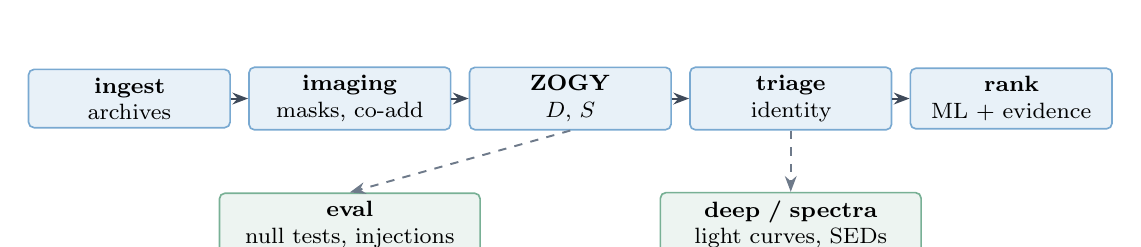
\begin{tikzpicture}[font=\footnotesize,
  b/.style={draw=accent!60,fill=accent2,line width=0.6pt,rounded corners=2pt,
    align=center,inner sep=3pt,text width=2.35cm},
  ar/.style={-{Stealth[length=2mm]},draw=slate,line width=0.7pt}]
  \node[b] (i) at (1.3,0) {\textbf{ingest}\\ archives};
  \node[b] (m) at (4.1,0) {\textbf{imaging}\\ masks, co-add};
  \node[b] (z) at (6.9,0) {\textbf{ZOGY}\\ $D$, $S$};
  \node[b] (t) at (9.7,0) {\textbf{triage}\\ identity};
  \node[b] (l) at (12.5,0) {\textbf{rank}\\ ML + evidence};
  \draw[ar] (i)--(m); \draw[ar] (m)--(z); \draw[ar] (z)--(t); \draw[ar] (t)--(l);
  \node[draw=good!60,fill=good!8,line width=0.6pt,rounded corners=2pt,align=center,
    inner sep=3pt,text width=3.1cm] (e) at (4.1,-1.6) {\textbf{eval}\\ null tests, injections};
  \node[draw=good!60,fill=good!8,line width=0.6pt,rounded corners=2pt,align=center,
    inner sep=3pt,text width=3.1cm] (d) at (9.7,-1.6) {\textbf{deep / spectra}\\ light curves, SEDs};
  \draw[ar,dashed,draw=muted] (z.south) -- (e.north);
  \draw[ar,dashed,draw=muted] (t.south) -- (d.north);
\end{tikzpicture}
\caption{Pipeline stages. Dashed links are optional products evaluated on the same cut-outs. One
JSON detection contract is shared by the batch and live paths, so a batch result and a served result
are byte-identical.}
\label{fig:pipeline}
\end{figure}

\subsection{Masking and co-addition}
Fourteen defect bits are rejected: cosmic-ray hits, saturation, hot and cold pixels, non-functional
channels, persistence, and statistical outliers. Two bits are deliberately preserved ---
\code{FULLSAMPLE} and \code{SOURCE} --- because rejecting \code{SOURCE} (bit 21) erased genuine
astronomical flux and produced artificial hollows around bright stars that mimic transients.

Masks are matched across epochs: a pixel masked in epoch 2 is also dropped in epoch 1, so a mask
hole cannot manufacture a dipole. Before co-addition each exposure receives sigma-clipped median
background subtraction, zodiacal-model removal and inverse-variance weighting,
$w_k = 1/\tilde V_k$, giving $\sigma_C^2 = \left(\sum_k w_k\right)^{-1}$.

\subsection{Proper subtraction}
ZOGY \cite{zogy} forms the difference and significance images
\begin{equation}
\hat D=\frac{\hat P_1\hat I_2-\hat P_2\hat I_1}
             {\sqrt{\sigma_1^2|\hat P_2|^2+\sigma_2^2|\hat P_1|^2}},
\qquad
S=\frac{\hat D\,\hat P_D}{\sqrt{\hat\sigma_1^2+\hat\sigma_2^2}},
\label{eq:zogy}
\end{equation}
where $\hat P_k$ and $\hat I_k$ are the Fourier transforms of the PSF and image for epoch $k$, and
$\sigma_k$ their noise. Nothing is fitted: each image is convolved with the other's PSF, and the
division by the combined noise makes $S$ unit-variance Gaussian wherever the sky is constant.
Empirical PSFs come from a $21\times21$ detector-zone grid selected by the cut-out's WCS. The cost is
two 2-D fast Fourier transforms per epoch pair --- under 0.6\,s for a $180^2$ frame.

\subsection{Detection statistics and threshold calibration}
For $N=180\times180=32\,400$ pixels the two-tailed Gaussian expectation is
$\mathbb{E}[N_{\rm FP}] = 2N^2\Phi(-\tau)$. At $\tau=5$ this predicts $0.0186$ false pixels per
frame; at $\tau=6$, $6.4\times10^{-5}$. Real co-adds are resampled onto a common grid, which
correlates neighbouring pixels and reduces the effective number of resolution elements, so the
empirical curve departs from the analytic one (Figure~\ref{fig:null}). Split-epoch null tests gave
$0.86$ false candidates per field at $5\sigma$ and $0.48$ at $6\sigma$; after the full triage chain
the residual is $1.66$ per field. We therefore adopt $\tau=6.0\sigma$ as the operating point, and
state the empirical, not the theoretical, false-alarm rate.

\begin{figure}[t]
\centering
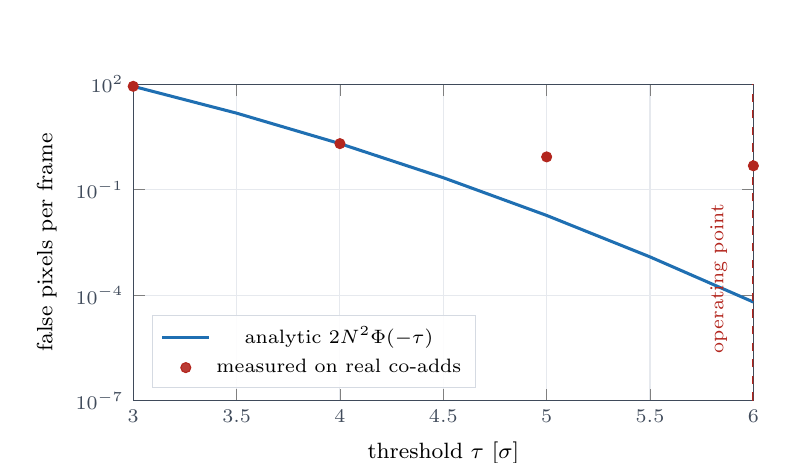
\begin{tikzpicture}[font=\footnotesize]
  \begin{axis}[width=0.78\linewidth,height=5.6cm,xmin=3,xmax=6,ymin=1e-7,ymax=1e2,ymode=log,
    xlabel={threshold $\tau$ [$\sigma$]},ylabel={false pixels per frame},
    tick label style={font=\scriptsize,text=slate},axis line style={slate},
    grid=major,grid style={rule!60},
    legend style={font=\scriptsize,draw=rule,at={(0.03,0.04)},anchor=south west,
      fill=white,fill opacity=0.9,text opacity=1}]
    \addplot[accent,line width=1.1pt] coordinates
      {(3,87.5) (3.5,15.1) (4,2.05) (4.5,0.220) (5,0.0186) (5.5,0.00123) (6,6.4e-5)};
    \addlegendentry{analytic $2N^2\Phi(-\tau)$}
    \addplot[only marks,mark=*,mark size=1.8pt,bad] coordinates
      {(3,87.5) (4,2.05) (5,0.86) (6,0.48)};
    \addlegendentry{measured on real co-adds}
    \draw[bad,dashed,line width=0.9pt] (axis cs:6,1e-7) -- (axis cs:6,1e2);
    \node[text=bad,font=\scriptsize,rotate=90,anchor=south] at (axis cs:5.92,3e-4)
      {operating point};
  \end{axis}
\end{tikzpicture}
\caption{Analytic and empirical false-pixel curves. The measured points exceed the Gaussian
prediction because co-addition and reprojection correlate pixels; the $6.0\sigma$ operating point is
chosen from the measured curve.}
\label{fig:null}
\end{figure}


\subsection{Morphology and physical pairing}
Significance peaks are grouped into candidate detections, and each is classified by geometry. A
\emph{dipole} --- a negative lobe and a positive lobe separated along a straight line --- indicates
displacement; dividing the separation by the elapsed time gives a proper motion. A single positive
\emph{monopole} indicates brightening; a single negative monopole indicates fading or occultation.

Two kinematic guards separate motion from variability. First, lobe separation must lie within the
maximum plausible proper motion over the actual baseline, $\Delta_{\rm px} \le \mu_{\max}\Delta t$;
this prevents a fading star from being paired with unrelated noise dozens of arcseconds away.
Second, the two lobes must agree in flux within a factor of two, and a flux-consistency metric
$\eta = |S_+ + S_-|/|S_+ - S_-|$ distinguishes pure displacement from combined motion and
variability.

\subsection{Identity: catalogue triage and asteroids}
Catalogue positions are quoted at their own epochs: Gaia DR3 at J2016.0, AllWISE at 2010.56. Over
the decade to the SPHEREx epoch a high-proper-motion star can move by $\sim$100 pixels, so every
catalogue position is propagated along its proper-motion vector to the exact exposure MJD before any
cone search. Match radii scale with brightness --- $10\arcsec$ for faint stars ($G\ge16$) up to
$120\arcsec$ for $G\le9$ --- with an outer $180\arcsec$ bright-star halo veto.

Detections are routed into six classes: \code{KNOWN\_MOVER}, \code{VARIABLE}, \code{STATIC\_CHANGED},
\code{BRIGHT\_STAR}, \code{MASK\_ARTEFACT} and \code{CANDIDATE}. Solar-system objects are identified
rather than guessed: every exposure timestamp is queried against JPL Horizons' small-body
identification service, enriched from the Small-Body Database and cross-checked geometrically
against CADC SSOIS inside a 25\,s time-box. If an external service is unreachable the card reports
the check as unavailable; it never defaults to ``candidate''.

\subsection{Ranking: calibrated ML and combined evidence}
A gradient-boosted classifier is trained on 12\,150 labelled examples (injections, catalogue sources
and split-epoch null residuals) using 22 engineered features: signal-to-noise, $\chi^2$ goodness of
fit, ellipticity, FWHM ratio, local noise ratio, masked fraction and related statistics. Isotonic
regression calibrates the score into a posterior, validated with field-wise GroupKFold plus four
held-out fields.

The classifier ranks; it never overrides a catalogue verdict. Five evidence streams are combined into
a believability score $s=\sum w_i v_i/\sum w_i$: calibrated ML probability ($w=0.40$), matched-filter
significance ($0.25$), kinematic consistency against NEOWISE and Gaia ($0.15$), asteroid clearance
($0.10$) and optical confirmation from NEOSSat ($0.10$). An unavailable stream reports a null weight
rather than zero, so an outage cannot masquerade as evidence against a candidate.

\subsection{Time-domain and spectroscopic products}
At the ecliptic poles the field is revisited $\sim$20\,800 times. Because the linear variable filter
maps wavelength to detector position, spacecraft roll changes the observed wavelength of a fixed
star, and raw photometry varies by tens of per cent for no physical reason. Each star's spectral
energy distribution is therefore modelled across all bands and divided out of every visit, with a 3\%
systematic floor, before variability tests.

The same wavelength solution yields a low-resolution spectrum per cut-out. Three indices --- methane
absorption near 1.6\,\textmu m, water at 1.5 and 2.0\,\textmu m, and the near-infrared slope ---
separate brown dwarfs, icy bodies and warm young stars. Below 30 usable bands the classifier abstains
and reports raw fluxes: a label that cannot be supported is worse than no label.


\section{Validation}
\label{sec:validation}

\subsection{The completeness defect and its correction}
An early version of the detector recovered only 0.2\% of planted sources under strict scoring. The
cause was architectural rather than parametric, and three corrections were required.

\emph{(1) Global normalisation.} The significance map was divided by a single frame-wide standard
deviation. A bright star with imperfect subtraction inflates that scale and suppresses every real
detection elsewhere in the frame. Replacing it with a median-absolute-deviation estimator restores
sensitivity.

\emph{(2) Unconstrained dipole pairing.} Any negative lobe was paired with any positive lobe within
$75\arcsec$ ($\sim$25 pixels), so fading stars were labelled movers. Constraining the pairing by
$\mu_{\max}\Delta t$ and a factor-two flux ratio removes those false pairs.

\emph{(3) Fixed bright-star mask.} A fixed $3\arcmin$ mask left the halo of $\epsilon$ Indi
unmasked, and its residual ring produced 44 false candidates in one field. A mask whose radius grows
exponentially with stellar brightness removes it.

Together these changes raised strict recovery from 0.2\% to 69.3\% (Figure~\ref{fig:recovery}) ---
a factor of 350, with no change to the underlying subtraction.

\subsection{Split-epoch null testing}
A detector's false-alarm rate can be measured without a truth table by constructing a sky whose true
answer is zero. Each visit is split into two interleaved halves and one is subtracted from the
other; both were taken minutes apart at the same pointing, so no genuine astrophysical change can
exist between them. Across 17 DR1 fields, 220 realisations and 3.57\,deg$^2$, raw subtraction
produced 8\,854 peaks. Catalogue matching, mask verification and halo vetoes reduced this to
$1.66$ false candidates per field, with exactly zero in six star fields (M31, Betelgeuse, M42,
Proxima Centauri, R Draconis, Sgr\,A$^*$).

\subsection{Strict injection--recovery}
Completeness was measured by planting 12\,240 synthetic sources in real co-adds, convolved with the
empirical PSF of the relevant detector zone, over six signal-to-noise levels (3--20) and four proper
motions (2--20$\arcsec$/yr) with random trajectory angles. A source counts as recovered only if it is
detected within 1.5 pixels of the injection position \emph{and} classified as the injected kind; a
mover recovered as a monopole is a failure.

Recovery is 96.7\% for brightening and 95.3\% for fading transients, and 56.0\% for moving dipoles
(Figure~\ref{fig:recovery}). The mover deficit is geometric: below $\sim$2$\arcsec$/yr the
displacement over six months is roughly one arcsecond --- a fraction of a pixel --- so the two lobes
overlap inside the PSF and partially cancel. Above $10\arcsec$/yr recovery is essentially complete.
Overall strict recovery is 69.3\%.

\begin{figure}[t]
\centering
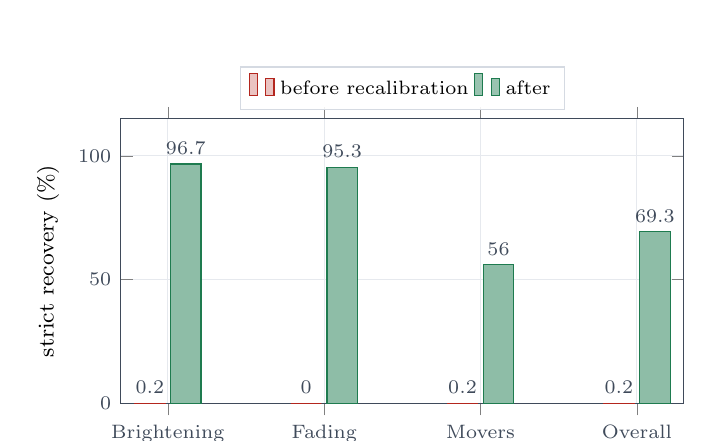
\begin{tikzpicture}[font=\footnotesize]
  \begin{axis}[width=0.72\linewidth,height=5.2cm,ybar,bar width=11pt,ymin=0,ymax=115,
    ylabel={strict recovery (\%)},
    symbolic x coords={{Brightening},{Fading},{Movers},{Overall}},
    xtick=data,tick label style={font=\scriptsize,text=slate},axis line style={slate},
    grid=major,grid style={rule!60},
    nodes near coords,nodes near coords style={font=\scriptsize\bfseries,text=slate},
    legend style={font=\scriptsize,draw=rule,at={(0.5,1.03)},anchor=south,legend columns=2,
      fill=white,fill opacity=0.9,text opacity=1}]
    \addplot[fill=bad!30,draw=bad] coordinates
      {({Brightening},0.2) ({Fading},0.0) ({Movers},0.2) ({Overall},0.2)};
    \addlegendentry{before recalibration}
    \addplot[fill=good!50,draw=good] coordinates
      {({Brightening},96.7) ({Fading},95.3) ({Movers},56.0) ({Overall},69.3)};
    \addlegendentry{after}
  \end{axis}
\end{tikzpicture}
\caption{Strict injection--recovery before and after the three corrections of
Section~\ref{sec:validation}. The mover class remains limited by PSF overlap at low proper motion,
not by the detector.}
\label{fig:recovery}
\end{figure}


\section{Results}
\label{sec:results}

\subsection{The census}
Across 18 fields the pipeline reports 109 detections at $6.0\sigma$: 99 \code{KNOWN} (91\%) and 10
\code{CANDIDATE} (9\%); see Figure~\ref{fig:census} and Table~\ref{tab:fields}. Detection count is
not discovery count. Sirius, M31, M104, M1 and Barnard's Star are fully explained by catalogued
proper motion, known variability, asteroid ephemerides or masked artefacts.

Two fields return nothing, and both are reported as such rather than adjusted until something
appears. M42 is a null sky: the nebular gas is stationary across the baseline. Sgr\,A$^*$ is refused
outright because the two epochs share no detector band, so no honest subtraction exists.

\begin{figure}[t]
\centering
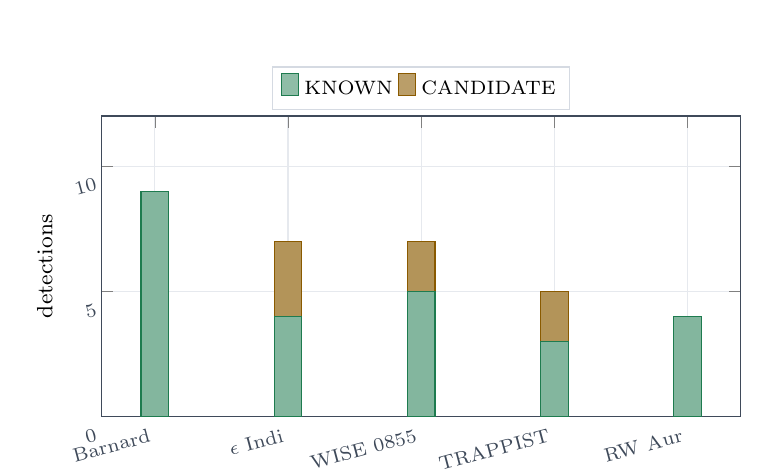
\begin{tikzpicture}[font=\footnotesize]
  \begin{axis}[width=0.8\linewidth,height=5.4cm,ybar stacked,bar width=10pt,ymin=0,ymax=12,
    ylabel={detections},
    symbolic x coords={{Barnard},{$\epsilon$ Indi},{WISE 0855},{TRAPPIST},{RW Aur}},
    xtick=data,tick label style={font=\scriptsize,text=slate,rotate=15,anchor=north east},
    axis line style={slate},grid=major,grid style={rule!60},
    legend style={font=\scriptsize,draw=rule,at={(0.5,1.02)},anchor=south,legend columns=2,
      fill=white,fill opacity=0.9,text opacity=1}]
    \addplot[fill=good!55,draw=good] coordinates
      {({Barnard},9) ({$\epsilon$ Indi},4) ({WISE 0855},5) ({TRAPPIST},3) ({RW Aur},4)};
    \addlegendentry{KNOWN}
    \addplot[fill=warn!65,draw=warn] coordinates
      {({Barnard},0) ({$\epsilon$ Indi},3) ({WISE 0855},2) ({TRAPPIST},2) ({RW Aur},0)};
    \addlegendentry{CANDIDATE}
  \end{axis}
\end{tikzpicture}
\caption{Detections for the five mandatory targets: 35 in total, of which seven remain unexplained.
The thirteen benchmarks contribute the remaining 74.}
\label{fig:census}
\end{figure}

\subsection{The ten candidates}
The ten residuals sit in five fields: $\epsilon$ Indi B (3), WISE 0855 (2), M45 (2), TRAPPIST-1 (2)
and 3C 273 (1). All are faint infrared excesses beyond the Gaia and WISE detection limits, in crowded
or high-background regions --- exactly the regime SPHEREx was designed to explore, and exactly the
regime where a candidate is a hypothesis rather than a discovery. Each carries its full evidence
breakdown so a follow-up observer can set the priority.

Barnard's Star illustrates the most instructive failure of the project. It was the first
``candidate'' the pipeline reported, and it was not a candidate at all but a coordinate-frame error:
Gaia's J2016.0 position was compared with a 2026 image without propagating the star's
$10.4\arcsec$/yr proper motion, a displacement of 94$\arcsec$. With epoch propagation the
$36.2\sigma$ dipole is matched as \code{KNOWN\_MOVER} and the field contains zero candidates.

\subsection{Variables and deep fields}
In fields containing catalogued AAVSO VSX variables, seven of 101 are recovered. This is a lower
bound rather than a failure rate: a catalogued variable need not change measurably during our
particular six-month window.

In a 78-visit north ecliptic pole dataset the variability pipeline flagged exactly one of six stars
as variable, and Gaia DR3 independently lists the same star. That is a single detection with no false
positives, the appropriate benchmark for a first deep-field run.


\section{Discussion}

\paragraph{What works.} The combination of an analytic null, an empirically calibrated threshold and
strict testing produces a detector whose behaviour can be stated in advance. The three corrections
of Section~\ref{sec:validation} are physical arguments, not hyperparameter choices, which is why the
improvement transferred to every field rather than to a tuning set.

\paragraph{Limitations.} Four deserve to be stated plainly. First, mover completeness at low proper
motion is limited by PSF overlap; the honest fix is a joint fit of position and flux across epochs
rather than a pairwise difference. Second, catalogue triage is limited by catalogue depth: an object
absent from Gaia and WISE is unexplained, not necessarily new. Third, the sample is 18 fields of two
epochs each, not the full mission --- scaling is a throughput question, not a methodological one.
Fourth, the classifier's headline precision is inflated by synthetic dipoles, and we therefore report
monopole-only skill (0.90/0.82 brightening, 0.72/0.63 fading).

\paragraph{Reproducibility as a design constraint.} Public data only, content-addressed snapshots and
a single JSON contract are not incidental conveniences: they are what allow a third party to re-run a
number in this paper and obtain the same answer.

\section{Conclusions}

SPHERExLens delivers an open, calibrated and reproducible difference-imaging pipeline for SPHEREx
DR1. On 18 fields and 246 cut-outs it reports 109 detections, explains 91\% of them with public
catalogues, recovers 69.3\% of 12\,240 injected sources under a strict criterion, and measures
$1.66$ false candidates per field in a null test whose true answer is zero. The detector design, the
calibration and the failure modes are documented together, because a candidate list is only as
useful as the statement of how often it is wrong.

\section*{Data and code availability}
All inputs are public: SPHEREx DR1 through NASA/IPAC IRSA (SIA2 and the \code{nasa-irsa-spherex}
S3 bucket), Gaia DR3, AllWISE/NEOWISE, AAVSO VSX, JPL Horizons and the Small-Body Database, and CADC
SSOIS. The pipeline ($\sim$21\,400 lines of runtime Python), the evaluation harness (null tests,
injection--recovery) and the browser interface ($\sim$7\,600 lines) are released with a JSON
detection contract and a 21-point security review; every figure here can be regenerated from the
published snapshots.

\begin{thebibliography}{99}\small

\bibitem{spherex} Dor\'e, O., et al.\ 2016, ``SPHEREx: an all-sky near-infrared spectral imager,''
JATIS, 2, 041206.

\bibitem{zogy} Zackay, B., Ofek, E.~O., \& Gal-Yam, A.\ 2016, ``Proper image subtraction --- optimal
transient detection, photometry and shape measurements,'' ApJ, 830, 27.

\bibitem{alard} Alard, C., \& Lupton, R.~H.\ 1998, ``A method for optimal image subtraction,''
ApJ, 503, 325.

\bibitem{bramich} Bramich, D.~M.\ 2008, ``A new algorithm for difference image analysis,''
MNRAS, 386, L77.

\bibitem{sfft} Hu, L., et al.\ 2022, ``SFFT: a fast image subtraction method for undersampled
images,'' ApJ, 936, 157.

\bibitem{gaia} Gaia Collaboration 2023, ``Gaia Data Release 3: summary of the content and survey
properties,'' A\&A, 674, A1.

\bibitem{wise} Mainzer, A., et al.\ 2011, ``Preliminary results from NEOWISE,'' ApJ, 731, 53.

\bibitem{vsx} Watson, C.~L., Henden, A.~A., \& Price, A.\ 2020, ``The International Variable Star
Index,'' AAS Meeting Abstracts, 52, 305.01.

\bibitem{antares} Smith, K.~W., et al.\ 2019, ``ANTARES: the Arizona-NOAO Temporal Analysis and
Response to Events System,'' arXiv:1907.06241.

\bibitem{alerce} F\"orster, F., et al.\ 2021, ``The Automatic Learning for the Rapid Classification
of Events pipeline,'' AJ, 161, 242.

\bibitem{lasair} Smith, K.~W., et al.\ 2019, ``Lasair: the transient alert broker for LSST:UK,''
RNAAS, 3, 26.

\bibitem{fink} M\"oller, A., et al.\ 2021, ``Fink, a new generation of broker for the LSST/Rubin
Observatory,'' MNRAS, 501, 3272.

\end{thebibliography}

\end{document}

surveys --- infrared: general --- astrometry}
